\documentclass[10pt]{article}
\usepackage{multicol}
\usepackage{authblk}
\usepackage{mathptmx}
\usepackage{graphicx}
\setlength{\columnsep}{5mm}
\usepackage{blindtext}
\usepackage{geometry}
\usepackage{url}
\usepackage{listings}
\usepackage{xcolor}
\usepackage{float}
\usepackage{longtable}


\definecolor{codegreen}{rgb}{0,0.6,0}
\definecolor{codegray}{rgb}{0.5,0.5,0.5}
\definecolor{codepurple}{rgb}{0.58,0,0.82}
\definecolor{backcolour}{rgb}{0.95,0.95,0.92}

\lstdefinestyle{mystyle}{
    backgroundcolor=\color{backcolour},   
    commentstyle=\color{codegreen},
    keywordstyle=\color{magenta},
    numberstyle=\tiny\color{codegray},
    stringstyle=\color{codepurple},
    basicstyle=\small,
    columns=flexible,
    breakatwhitespace=false,         
    breaklines=true,                 
    captionpos=b,                    
    keepspaces=true,                 
    numbers=left,                    
    numbersep=2pt,                  
    showspaces=false,                
    showstringspaces=false,
    showtabs=false,                  
    tabsize=2
}

\lstset{style=mystyle}

\geometry{
  a4paper,
  left = 20mm,
  top = 2mm,
  right = 20mm
}

\title{\textbf{Parallel dragonfly algorithm} %
  \\[2ex] \large High Performance Computing for Data Science course 2024/2025}

\author[1]{Mattia Santaniello}
\author[2]{Alessio Zeni}
\affil{University of Trento}

\begin{document}

\maketitle

\begin{multicols}{2}[\fontsize{9}{9}\section*{Abstract} \textbf{Dragonfly algorithm is a new kind of approach used to solve optimization problems through the emulation of dragonflies movements, but it lacks scalability. In this paper the authors try to set up an approach based on parallelization thanks to the use of API for high performance computing like MPI and OpenMP, then there will be a comparison of execution times between presented implementation and the classic approach based on serial programming, in order to see if parallelization could lead to a performance improvement and possible future extensions.}\newline]

\section{Introduction}

Recent years have seen the raise and evolution of swarm intelligent algorithms, based on meta-heuristic approach where single individuals of a complex population follow an exploration-exploitation methodology to find the best solution in their local search space; each member of the group work independently from the others, leading to a subdivision of the labour which decrease the overall amount of execution time, working as decentralized and parallel units; but also, due to the fact that they mimic the behaviour of biological life forms, it is possible then that they could generate random patterns through the interaction with each other.  The dragonfly algorithm has been proposed for the first time in 2016, and its purpose is to simulate the behaviour of a dragonfly population according to the principles of swarm intelligent algorihms seen previously. It has gained more and more popularity: it is in estimated that during 2019 more than 300 scientific papers cited the algorithm \cite{DASurvey}, due to the fact that it has demonstrated some characteristics similar to other algoritms of the same kind, however in contrast with other swarm intelligent algorithms however it present less probability to be trapped into a local optima \cite{DAReview}. This paper aims to define a new approach based on popular parallel APIs, and also trying to understand if parallelization could lead to a significant speed up in performances that can be considered by future researches on this algorithm 

\subsection*{How the algorithm works}
The execution begins with the initialization of some arrays which are the position $P$ of all dragonfiles and the `step` vector $\Delta P$ representing the velocities of each single individual,the position of source foods $F$ and the position of enemies $E$; then the algorithm executes an iteration loop where, for each dragonfly, we calculate some coefficient that will be used to update the internal state of the program. This procedure is simulated through the observation of repetitive patterns observed in the behaviour of dragonflies, which are:



\begin{itemize}
  \item Alignment of their velocity with other members of the same group, given by the formula  $A_i = \frac{\sum^M_{j=1}V_j}{M}$, where $V_j$ is the velocity of the j-th neighbour

  \item Separation of single members in order to avoid collision, and it is retrieved by the equation  $S_i = - \sum^M_{j=1}{P - P_j}$, where $P_j$ is the position of the j-th neighbour and $P$ the current individual position.
    
  \item Cohesion towards the center of the group, given by $C_i = \frac{\sum^M_{j=1}P_j}{M} - P$ 
  \item Attraction to a common source food, expressed by the formula $ F_i = F^+ - P$, where $F^+$ is the position of the current prey and $P$ is the position of the current dragonfly
  \item Distraction of enemies, represented by the equation $ E_i = E^- - P$ where $E^-$ is the position of the current enemy 
\end{itemize}

\noindent Once all the parameters have been calculated we can now update the current step vector of each dragonfly using the following equation: $$\Delta P^{t+1}_{i} = (sS_i + aA_i + fF_i + cC_i) + \omega\Delta P^t_i$$ where $s,a,f,c$ are respectevly the separation weight, the alignment weight, the attraction weight, the cohesion weight and $\omega$ is the inertia weight, all of them are randomly chosen in the interval $[0,1]$. When all step vectors have been updated we can now set the new position of the dragonflies using this equation, which takes the new step vector as an input: $$P^{t+1}_{i} = P_i^t + \Delta P_{i}^{t+1}$$. However if there is a dragonfly which does not have any neighbour then we assume that the overall population moves in a random way: the most common method to do that is to use a random walk function. The previous formula then must be modified into this one here: $$P^{t+1}_i = P_i^t + Levy(d)$$ where $d$ is the dimension of the position vector, and $Levy(d)$ is the Levy flight function, which is calculated in this way: $$Levy(d) = 0.01\times\frac{r_1 \times \sigma}{|r_2|^{\frac{1}{\beta}}}$$ where $r1$ and $r2$ are two random numbers uniformally distributed in the interval $[0,1]$, and $\sigma$ is a vector calculated using the following formula: $$\sigma = \frac{sin(\frac{\beta\pi}{2})\times\Gamma(1+\beta)}{\Gamma(\frac{\beta+1}{2})\times \beta \times 2^{(\beta-1)/2}}$$ where $\Gamma(x)$ is the gamma function \cite{WikiGamma}, and $\beta$ is a constant.Another valid approach is to apply, instead of Levy flight, the brownian motion model, used especially in gas and particle analysis: this seems to return better performances \cite{BDragonfly}. 

\section{first approach}

Now that we have seen the overall procedure it is possible to write a naive implementation of the algorithm in order to 
have a base for further developments. An example of the implementation can be observed in the following code snippet:


\begin{lstlisting}[language=C,caption={first implementation of the dragonfly algorithm}]
  void dragonfly_algorithm(Dragonfly *d,
                          float *average_speed, 
                          float *cumulated_pos, 
                          float * food, 
                          float * enemy, 
                          unsigned int N) {

    unsigned int dim = d->dim;
      // for each dragonfly
    for (unsigned int j = 0; j < d->N; j++) {
      float *cur_pos = d->positions + dim * j;
      float *cur_speed = d->speeds + dim * j;

      // compute separation: Si = -sumall(X-Xi)
      memcpy(d->S, cumulated_pos, sizeof(float) * dim);
      scalar_prod_assign(d->S, 1.0/(float)N, dim);
      sub_assign(d->S, cur_pos, dim);
      scalar_prod_assign(d->S, d->w.s, dim);

      // compute alignament: Ai = avarage(Vi)
      memcpy(d->A, average_speed, sizeof(float) * dim);
      scalar_prod_assign(d->A, d->w.a, dim);

      // compute cohesion: Ci = avarage(Xi)-X
      memcpy(d->C, cumulated_pos, sizeof(float) * dim);
      scalar_prod_assign(d->C, 1.0 / (float)N, dim);
      sub_assign(d->C, cur_pos, dim);
      scalar_prod_assign(d->C, d->w.c, dim);

      // food attraction: Fi=X_food - X
      memcpy(d->F, food, sizeof(float) * dim);
      sub_assign(d->F, cur_pos, dim);
      scalar_prod_assign(d->F, d->w.f, dim);

      // enemy repulsion: E=X_enemy+X
      memcpy(d->E, enemy, sizeof(float) * dim);
      sum_assign(d->E, cur_pos, dim);
      scalar_prod_assign(d->E, d->w.e, dim);

      brownian_motion(d->levy, dim, &d->seed);


      // compute speed = sSi + aAi + cCi + fFi + eEi + w
      scalar_prod_assign(cur_speed, d->w.w, dim);
      sum_assign(cur_speed, d->E, dim);
      sum_assign(cur_speed, d->F, dim);
      sum_assign(cur_speed, d->C, dim);
      sum_assign(cur_speed, d->A, dim);
      sum_assign(cur_speed, d->S, dim);
      sum_assign(cur_speed, d->levy, dim);

      // update current pos
      sum_assign(cur_pos, cur_speed, dim);
    }

    // update weights
    weights_step(&d->w);
  }
\end{lstlisting}

\noindent After the initialization of velocities and positions of agents,
which will be represented by two separated matricies with the same dimension equal to the number of members of our
population times the dimension of our problem, the algorithm starts to execute a for loop with a fixed amount of iteration stored in the variable $d\rightarrow N$, 
and will repeatetly compute the following steps:
\begin{itemize}
  \item retrieve current speed and position of the j-th dragonfly
  \item compute separation, alignment, cohesion, food attraction and enemy distraction vectors,
  stored into arrays placed in the struct Dragonfly
  \item calculate product between weigths and arrays
  \item update speed and position the dragonfly considering also levy flight
\end{itemize}
\subsection*{chunks}
We can improve this approach introducing groupments of dragonflies into chunks, 
allowing us to calculate local minima of different areas and compare them in order
to get as close as possible to the global minima. which will be considered
autonomous agents that will calculate local minima of our fitness function, updating then the 
global status of by sending messages to all other dragonfly chunks. 

\begin{figure}[H]
  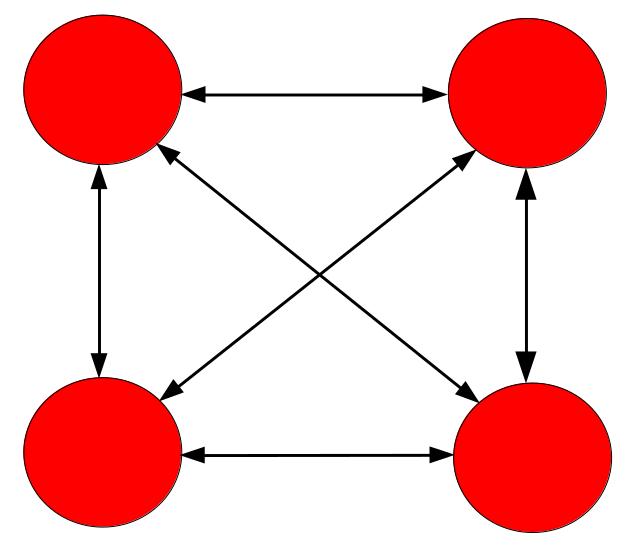
\includegraphics[scale=0.3]{chunks.png}
  \caption{illustration of communication between chunks}
\end{figure}


\section{Performace tests}

The serial implementation seen above can be easily tried out using some test function 
with known global minima in order to check the overall performances. We need to 
report time execution for each test function, using the input dimension as independent variable;
since however we have multiple input parameters to compare, we also have to decide which one will 
be considered during the performance evaluation.

\begin{table}[H]
\begin{tabular}{| c | c | c | c |}
  \hline
  \textit{Nr of iterations} & \textbf{sphere [ms]} & \textbf{rosenblock [ms]} & \textbf{rastrigin [ms]}\\
  \hline
  10 \\
  \hline

  100 \\
  \hline

  1000 \\
  \hline

  10000 \\ 
  \hline

  100000 \\
  \hline
\end{tabular}

\end{table}

\begin{table}[H]
  \begin{tabular}{| c | c | c | c |}
    \hline
    \textit{Nr of iterations} & \textbf{sphere [ms]} & \textbf{rosenblock [ms]} & \textbf{rastrigin [ms]}\\
    \hline
    10 \\
    \hline
  
    100 \\
    \hline
  
    1000 \\
    \hline
  
    10000 \\ 
    \hline
  
    100000 \\
    \hline
  \end{tabular}
\end{table}

\noindent As we can see the execution time increases exponentially with the consequentially increase of
the input.

\section{Parallel implementation}

\section{Parameters Retrievement}

\section{Speedup and final conclusions}

\end{multicols}

\bibliographystyle{unsrt}
\bibliography{references}


\end{document}
